% Intended LaTeX compiler: pdflatex
\documentclass[11pt]{article}
\usepackage[utf8]{inputenc}
\usepackage[T1]{fontenc}
\usepackage{graphicx}
\usepackage{longtable}
\usepackage{wrapfig}
\usepackage{rotating}
\usepackage[normalem]{ulem}
\usepackage{amsmath}
\usepackage{amssymb}
\usepackage{capt-of}
\usepackage{imakeidx}
\makeindex[intoc]
\usepackage{times}
\usepackage{hyperref}
\hypersetup{
  colorlinks=true
}
\author{dparker}
\date{\today}
\title{roam2doc parse of /home/dparker/projects/roam2doc/tests/org\_files/examples/all\_nodes.org}
\setcounter{secnumdepth}{6}
\setlength{\parindent}{0pt}
\setcounter{tocdepth}{6}
\begin{document}
\maketitle
\tableofcontents
\clearpage
\section{The File \index{  The File}  (xref-id:3)  }
 \label{obj-3}
 \label{obj-2}
\section{Heading Level 1 \index{ Heading Level 1}  (xref-id:6)  }
 \label{obj-6}
 \label{obj-5}
\subsection{Heading Level 2 \index{ Heading Level 2}  (xref-id:9)  }
 \label{obj-9}
 \label{obj-8}
\subsubsection{Heading Level 3 \index{ Heading Level 3}  (xref-id:12)  }
 \label{obj-12}
 \label{obj-11}
\section{Section 1 heading \index{ Section 1 heading}  (xref-id:15)  }
 \label{obj-15}
 \label{obj-14}
\subsection{Section 1 subsection 1 heading and it has \textbf{\emph{some}} \texttt{objects} \index{ Section 1 subsection 1 heading and it has some  objects}  (xref-id:18)  }
 \label{obj-18}
 \label{obj-17}
\subsubsection{level 3 section \index{ level 3 section}  (xref-id:24)  }
 \label{obj-24}
 \label{obj-23}
\paragraph{level 4 section \index{ level 4 section}  (xref-id:27)  }
 \label{obj-27}
 \label{obj-26}
\subparagraph{level 5 section \index{ level 5 section }  (xref-id:30)  }
 \label{obj-30}
 \label{obj-29}
\begin{enumerate}
\item level 6 section \index{ level 6 section }  (xref-id:33) 
 \label{obj-33}
 \label{obj-32}
\end{enumerate}
\textbf{level 7 section After level 6,}\newline
letex will not consider it document structure, just text
\vspace{\baselineskip}

\section{Section 2 heading \index{ Section 2 heading}  (xref-id:42)  }
 \label{obj-42}
 \label{obj-41}
\begin{quote}
\end{quote}

This will be a paragraph.
This continues the paragraph. This sentence ends contains a
\emph{target}
\label{obj-50} (xref-id:50)
which is not visible but can be linked. See the
\hyperref[obj-385]{\textbf{links table} (xref:52)}
at the end of the document.  The next line (blank) will end the
paragraph.

This will be a second paragraph. 
The following blank lines will end it.
The following next two blank will also be part of the paragraph.
They should be part of the section directly.

a link
\hyperref[obj-161]{link to last line of the definition list later in the page (xref:63)}

\vspace{\baselineskip}
This will be a third paragraph and will have no extra blank lines before the next section.

\subsection{Subsection 1 Lists \index{ Subsection 1 Lists}  (xref-id:69)  }
 \label{obj-69}
 \label{obj-68}
\subsubsection{Ordered List \index{ Ordered List}  (xref-id:72)  }
 \label{obj-72}
 \label{obj-71}

 (xref-id:75)
\begin{enumerate} \label{obj-75}
\item
some
\textbf{bold}
text
\item
some
\emph{italic}
text
\begin{enumerate}
\item
External link
\href{http://example.com}{http://example.com}
\item
External link same as above, but with display text
\href{http://example.com}{same old thing}
\item
Internal link to something with a
\texttt{\#+NAME:}
keyword
\hyperref[obj-385]{Link the links table at the end (xref:97)}
\item
Internal link to a target
\hyperref[obj-384]{link to target "before\_links\_table" (xref:101)}
\item
Internal link to a heading by heading text
\hyperref[obj-381]{End Section (xref:105)}
\end{enumerate}
\end{enumerate}
\subsubsection{Unordered List \index{ Unordered List}  (xref-id:108)  }
 \label{obj-108}
 \label{obj-107}
\begin{itemize}
\item
first uitem
\item
second uitem
\item
third uitem
\item
third uitem
\begin{itemize}
\item
third uitem first subitem (actually a new list contained by third uitem)
\item
third uitem second subitem
\end{itemize}
\end{itemize}
\subsubsection{Definition List, this section has a properties drawer and the ID "foo\_bar\_section" \index{ Definition List, this section has a properties drawer and the ID "foo\_bar\_section"}  (xref-id:125)  }
 \label{obj-125}
 \label{obj-124}
\begin{description}
\item[Joe]
a fella`
\item[Joey]
a good fella
\end{description}
\subsubsection{List with type changing on nesting \index{ List with type changing on nesting}  (xref-id:137)  }
 \label{obj-137}
 \label{obj-136}
\begin{itemize}
\item
unordered list starts
\begin{itemize}
\item
unordered sub 1
\begin{itemize}
\item
unordered sub 1 subsub 1
\end{itemize}
\item
unordered sub 2
\textbf{bold text}
\end{itemize}
\item
unordered second 
\begin{description}
\item[foobar]
see a pattern?
\item[beebop]
arubop
\label{obj-161} (xref-id:161)
  Some text as a paragraph in an item!!! (this is child of unordered secont)
and a link
\hyperref[obj-15]{\textbf{\emph{back to the top!}} (xref:165)}
  and an embedded table!!

\begin{tabular}{|c|c|}
\hline
 xx  & \textbf{this item is bold} \\
 yy  & \emph{this item is italian} \\
\hline
\end{tabular}
\end{description}
\item
unordered third
\begin{enumerate}
\item
ordered first, child of unordered third
\begin{enumerate}
\item
THIS GETS PLACED IN WRONG PARENT!!!!!!
\end{enumerate}
\item
???
\end{enumerate}
\vspace{\baselineskip}
\vspace{\baselineskip}
\end{itemize}
\vspace{\baselineskip}
\subsubsection{List with a checkbox, we don't do anything with it \index{ List with a checkbox, we don't do anything with it}  (xref-id:195)  }
 \label{obj-195}
 \label{obj-194}
\begin{enumerate}
\item
inside
\item
done
\vspace{\baselineskip}
\vspace{\baselineskip}
\end{enumerate}
\section{Section 3 heading, more lists \index{ Section 3 heading, more lists}  (xref-id:205)  }
 \label{obj-205}
 \label{obj-204}
\subsection{Section 3-1 heading \index{ Section 3-1 heading}  (xref-id:208)  }
 \label{obj-208}
 \label{obj-207}
\begin{enumerate}
\item
List 1
\begin{enumerate}
\item
List 1 sub 1 (last item in list)
\end{enumerate}
\end{enumerate}
\subsection{Section 3-2 heading (causes end of above list) \index{ Section 3-2 heading (causes end of above list)}  (xref-id:217)  }
 \label{obj-217}
 \label{obj-216}
this first text should be in Section 2-2 before list' )

\begin{itemize}
\item
List 2
\begin{itemize}
\item
List 2 sub 1
\begin{enumerate}
\item
List 2 sub 1 sub list change type
      this should be para 1 line 1 inside List 2 sub 1 sub 1
      this should be para 1 line 2 inside List 2 sub 1 sub 1
      this should be para 1 line 3 inside List 2 sub 1 sub 1

\vspace{\baselineskip}
      this should be para 2 line 1 inside List 2 sub 1 sub 1
      this should be para 2 line 2 inside List 2 sub 1 sub 1
      this should be para 2 line 3 inside List 2 sub 1 sub 1 (last in list)
\vspace{\baselineskip}

\end{enumerate}
\end{itemize}
\end{itemize}
\section{Section 4 heading, tables \index{ Section 4 heading, tables}  (xref-id:241)  }
 \label{obj-241}
 \label{obj-240}
\subsection{A simple table \index{ A simple table}  (xref-id:244)  }
 \label{obj-244}
 \label{obj-243}
\begin{tabular}{|c|c|c|}
\hline
 row1-1  &  row1-2  &  row1-3  \\
 row2-1  &  row2-2  &  row2-3  \\
 row3-1  &  row3-2  &  row3-3  \\
\hline
\end{tabular}
\vspace{\baselineskip}
\subsection{A simple table with objects in some cells \index{ A simple table with objects in some cells}  (xref-id:270)  }
 \label{obj-270}
 \label{obj-269}
\begin{tabular}{|c|c|}
\hline
 a  & \textbf{1 bold item} \\
 b  & \emph{2 italian items} \\
 c  & \sout{3 other items} \\
 d  & a link inside a cell! -\textgreater{} \hyperref[obj-42]{see: section 2 (xref:293)} \\
\hline
\end{tabular}
\vspace{\baselineskip}
\section{Section 5 heading, text objects \index{ Section 5 heading, text objects}  (xref-id:297)  }
 \label{obj-297}
 \label{obj-296}
this text is in section 5

\textbf{bold text}

\emph{italic text}

\underline{underlined text}

\sout{line-through text}

\textbf{\emph{\sout{bold italic strikethrough}}}

\vspace{\baselineskip}
\texttt{monospace text}

\section{Section 6 heading, blocks \index{ Section 6 heading, blocks}  (xref-id:317)  }
 \label{obj-317}
 \label{obj-316}
\begin{itemize}
\item
These first two are "greater elements", so they can contain stuff
\begin{center}
A center block with a table inside

\begin{tabular}{|c|c|}
\hline
 ww  & Checking inside center block \textbf{this item is bold} \\
\hline
\end{tabular}
\end{center}
\item
A list
\begin{enumerate}
\item
Yeah

\begin{quote}
A quote block with a cite and  a table and list inside

 (xref-id:341)
 \label{obj-341}
\begin{tabular}{|c|c|}
\hline
 ww  & Checking inside quote \textbf{this item is bold} \\
\hline
\end{tabular}
\end{quote}
\end{enumerate}
\item
A list
\begin{enumerate}
\item
Yeah

\begin{verbatim}
This is an example
lines.append(" of what don't know")
\end{verbatim}
\begin{verbatim}
def foo():
return goodness
\end{verbatim}
\begin{verbatim}
I have things to say
and they should be heard!
\end{verbatim}
\begin{verbatim}
export blocks make little sense after conversion 
\end{verbatim}
\vspace{\baselineskip}
\end{enumerate}
\end{itemize}
\section{Section 7 heading, images \index{ Section 7 heading, images}  (xref-id:360)  }
 \label{obj-360}
 \label{obj-359}

 (xref-id:363)
\begin{enumerate} \label{obj-363}
\item
\begin{figure} [ht]
\centering
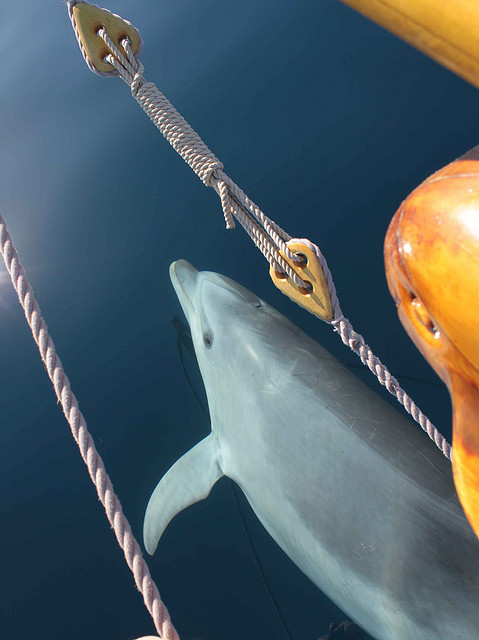
\includegraphics[width=\textwidth]{/home/dparker/projects/roam2doc/tests/org_files/examples/dolphin.jpg}
\caption{alt\_text}
\end{figure}
\item
\begin{figure} [ht]
\centering
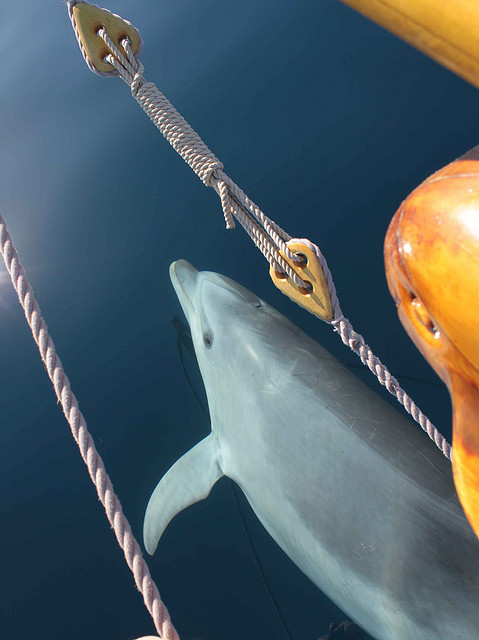
\includegraphics[width=\textwidth]{/home/dparker/projects/roam2doc/tests/org_files/examples/dolphin.jpg}
\caption{alt\_text\_2}
\end{figure}
\vspace{\baselineskip}
\end{enumerate}
\section{Include section \index{ Include section}  (xref-id:370)  }
 \label{obj-370}
 \label{obj-369}
\subsection{This section is from an included file! \index{ This section is from an included file!}  (xref-id:373)  }
 \label{obj-373}
 \label{obj-372}
\vspace{\baselineskip}
\subsubsection{This section is from a second included file! \index{ This section is from a second included file!}  (xref-id:377)  }
 \label{obj-377}
 \label{obj-376}
\vspace{\baselineskip}
\section{End Section \index{ End Section}  (xref-id:381)  }
 \label{obj-381}
 \label{obj-380}
\label{obj-384} (xref-id:384)

 (xref-id:385)
 \label{obj-385}
\begin{tabular}{|c|c|}
\hline
 Next cell points to paragraph 1 in list 1 under section 2  & \hyperref[obj-50]{link to paragraph1 (xref:390)} \\
 Next cell points to list1 under section 2                  & \hyperref[obj-75]{link to list 1 (xref:396)} \\
 Next cell points to a heading by text reference            & \hyperref[obj-15]{link to section 1 \textbf{with some bold text!} (xref:402)} \\
 Next cell has an unresolvable link                         & \textit{!!! link target "flabist" not found !!!} \\
\hline
\end{tabular}
\vspace{\baselineskip}
\vspace{\baselineskip}
\printindex
\noindent
\section*{Index}
\subsection*{Referenced Objects}
\small
\renewcommand{\arraystretch}{1.2}
\raggedright
\begin{tabular}{|p{3cm}|p{10cm}|}
\hline
\textbf{Referenced Object} & \textbf{Referenced by} \\
\hline
\hyperref[obj-50]{50} & 390  \\
\hyperref[obj-75]{75} & 396  \\
\hyperref[obj-161]{161} & 63  \\
\hyperref[obj-384]{384} & 101  \\
\hyperref[obj-385]{385} & 52,97  \\
\hyperref[obj-381]{381} & 105  \\
\hyperref[obj-15]{15} & 165,402  \\
\hyperref[obj-42]{42} & 293  \\
\hline
\end{tabular}
\end{document}